%
% Complete documentation on the extended LaTeX markup used for Insight
% documentation is available in ``Documenting Insight'', which is part
% of the standard documentation for Insight.  It may be found online
% at:
%
%     http://www.itk.org/

\documentclass{InsightArticle}

\usepackage{natbib}
\usepackage{amsfonts}
\usepackage[greek,german,english]{babel}
\usepackage{times}
\usepackage{subfigure}
%
% some definitions
%

\newcommand{\x}{\mathbf{x}}  %location-vector
\newcommand{\vi}{\mathbf{i}}  %location-vector
\newcommand{\vc}{\mathbf{c}}  %location-vector
\newcommand{\vx}{\mathbf{x}} %vector x
\newcommand{\va}{\mathbf{a}} %vector a
\newcommand{\vb}{\mathbf{b}} %vector b
\newcommand{\g}{\mathbf{g}}  %vector g
\newcommand{\n}{\mathbf{n}}  %vector n
\newcommand{\h}{\mathbf{h}}  %vector h
\newcommand{\vJ}{\mathbf{J}}  %vector J
\newcommand{\Real}{\mathbb{R}}  %Real Numbers
\newcommand{\Z}{\mathbb{Z}}  %Real Numbers
\newcommand\nR{\n_\epsilon(R,\x)}  %Reference NGF
\newcommand\nS{\n_\epsilon(S,\x)}  %Test      NGF
\newcommand\F{\mathfrak{F}} %Selected sequence similarity profile
\newcommand{\Fc}{\ensuremath{F_{\text{NGF}}} }   % Cost NGF general
\newcommand{\Fcs}{\ensuremath{{F_{\text{NGF}}^{(\cdot)}}} } % Cost NGF dot
\newcommand{\Fcc}{\ensuremath{{F_{\text{NGF}}^{(\times)}}} } % Cost NGF scalar
\newcommand{\Fcd}{\ensuremath{{F_{\text{NGF}}^{(\Delta\cdot)}}} } % Cost NGF scalar
\newcommand{\Fd}{\ensuremath{{F_{\text{NGF}}^{(\Delta)}}} } 
\newcommand{\Fdd}{\ensuremath{{F_{\text{NGF}}^{(\Delta^2)}}} } 
\newcommand{\Fssd}{\ensuremath{F_{\text{SSD}}} } % Cost SSD
\newcommand{\Domain}{\ensuremath{\Omega} }      % Image domain
\newcommand{\Range}{\ensuremath{\mathbb{V}} }   % Image intesnity range
\newcommand{\TDomain}{\ensuremath{\Theta} }     % Transformation space
\newcommand{\iref}{i_{\text{ref}}}               % Reference image index
\newcommand{\Iref}{\ensuremath{I_{\text{ref}}} } % Reference Image
\newcommand{\I}{\mathfrak{J}}                       % Image series
\newcommand{\Iphase}{\ensuremath{\I}' } % Phase aligned subset
\newcommand{\Iphasereg}{\ensuremath{\hat{\I}}' } % Registered phase aligned subset
\newcommand{\Ireg}{\hat{\I}}                       % Registered image series
\newcommand{\Syntset}{\mathfrak{R}}
\newcommand{\Treg}{T_{\text{reg}}}

\newcommand{\crate}{\ensuremath{c_{\text{rate}}} }
\newcommand{\Fsum}{\ensuremath{F_{\text{Sum}}} }

\newcommand{\avg}[1]{\ensuremath{E(#1)}}

\newcommand{\Cref}[1]{\ensuremath{{K^{(#1)}_{\text{ref}}}}}
\newcommand{\Creg}[1]{\ensuremath{{K^{(#1)}_{\text{reg}}}}}
\newcommand{\Corg}[1]{\ensuremath{{K^{(#1)}_{\text{org}}}}}

\newcommand{\Chref}[1]{\ensuremath{{\hat{K}^{(#1)}_{\text{ref}}}}}
\newcommand{\Chreg}[1]{\ensuremath{{\hat{K}^{(#1)}_{\text{reg}}}}}
\newcommand{\Chorg}[1]{\ensuremath{{\hat{K}^{(#1)}_{\text{org}}}}}
\newcommand{\noise}{\ensuremath{\eta} }

\newcommand{\changed}[1]{#1}
%\newcommand{\changed}[1]{\textbf{#1}}

\newcommand{\Time}{\ensuremath{\Theta}}
\newcommand{\Sec}{\ensuremath{\mathbb{S}} }
%\newcolumntype{k}{D{.}{.}{-1}}

\newcommand{\NGFKernel}{\code{NGFKernel} }
\newcommand{\NGFCross}{\code{NGFCrossKernel} }
\newcommand{\NGFScalar}{\code{NGFScalarKernel} }
\newcommand{\NGFScDelta}{\code{NGFScaledDeltaKernel} }
\newcommand{\NGFDelta}{\code{NGFDeltaKernel} }
\newcommand{\NGFDeltaB}{\code{NGFDelta2Kernel} }
\newcommand{\NGFMetric}{\code{NormalizedGradientFieldImageToImageMetric} }
\newcommand{\ImageToNGFFilter}{\code{ImageToNGFFilter} }
\newcommand{\scalar}[2]{\ensuremath{\langle #1, #2 \rangle} }

%\newcommand{\tiw}{p{0.15\columnwidth}}
\newcommand{\tabimage}[1]{\parbox[c]{1em}{\resizebox{0.15\columnwidth}{!}{#1}}}

\usepackage{graphicx}

%%%%%%%%%%%%%%%%%%%%%%%%%%%%%%%%%%%%%%%%%%%%%%%%%%%%%%%%%%%%%%%%%%
%
%  hyperref should be the last package to be loaded.
%
%%%%%%%%%%%%%%%%%%%%%%%%%%%%%%%%%%%%%%%%%%%%%%%%%%%%%%%%%%%%%%%%%%
\usepackage[bookmarks,
bookmarksopen,
backref,
colorlinks,linkcolor={blue},citecolor={blue},urlcolor={blue},
]{hyperref}


%  This is a template for Papers to the Insight Journal. 
%  It is comparable to a technical report format.

% The title should be descriptive enough for people to be able to find
% the relevant document. 
\title{An ITK implementation of the Normalized Gradient Field Image to Image Metric}

% 
% NOTE: This is the last number of the "handle" URL that 
% The Insight Journal assigns to your paper as part of the
% submission process. Please replace the number "1338" with
% the actual handle number that you get assigned.
%
\newcommand{\IJhandlerIDnumber}{3150}



% Increment the release number whenever significant changes are made.
% The author and/or editor can define 'significant' however they like.
\release{0.00}

% At minimum, give your name and an email address.  You can include a
% snail-mail address if you like.
\author{Gert Wollny, Maria J.~Ledesma-Carbayo, and Andres~Santos}
\authoraddress{Ciber BBN, Spain; \\
    Biomedical Imaging Technologies, 
    Department of Electronic Engineering, ETSIT, Universidad Politécnica de Madrid, Spain}

\begin{document}

%
% Add hyperlink to the web location and license of the paper.
% The argument of this command is the handler identifier given
% by the Insight Journal to this paper.
% 
\IJhandlefooter{\IJhandlerIDnumber}

\maketitle


\ifhtml
\chapter*{Front Matter\label{front}}
\fi


% The abstract should be a paragraph or two long, and describe the
% scope of the document.
\begin{abstract}
\noindent
This article describes the ITK implementation of a \emph{Normalized Gradient Fields} (NGF) based 
  image-to-image metric.
Some properties of the metric are discussed and example registrations are presented.
\end{abstract}

\IJhandlenote{\IJhandlerIDnumber}

\tableofcontents


\section{Introduction}

In an image registration framework, the choice of the right image similarity measure is important 
  to achieve a good image registration. 
Image similarity measures like the \emph{Sum of Squared Differences} (SSD), \emph{Cross Correlation}, and 
  \emph{(Normalized) Mutual Information} \cite{Maes97,Viola1997}, 
  are global measures that best describe the similarity of the image content, 
  if the material-intensity mapping is consistent over the whole image domain.
In image series, where the material-intensity mapping changes locally over time, like e.g., in perfusion 
  magnetic resonance imaging, these measures may not perform well.
Here, a similarity measure that draws its value only from a local vicinity of each pixel may 
  be more appropriated.

\section{A normalized gradient fields based image to image metric}
\label{sec:ngfmath}

Haber and Modersitzki \cite{haber05} proposed \emph{Normalized Gradient Fields} NGF as 
  an alternative image registration metric: 
Given a domain $\Domain$, an intensity range $\Range$, an image as a mapping $I: \Domain \rightarrow \Range$ 
  and its noise level \noise, a measure $\epsilon$
  for boundary ``jumps'' (locations with a high gradient) can be defined as
\begin{equation}
	\label{eq:epsilon}
	\epsilon := \eta \frac{ \int_{\Omega}  | \nabla I(\x) | d\x}{\int_{\Omega} d\x},
\end{equation}

\noindent
and with
\begin{equation}
	\label{eq:normeps}
       \| \nabla I(\x)\|_\epsilon := \sqrt{\sum_{i=1}^d \left(\nabla I(\x)\right)_i^2 + \epsilon^2},
\end{equation}

\noindent
the NGF of an image $I$ is defined as follows:
\begin{equation}
	\label{eq:ngf}
	\n_\epsilon(I, \x) := \frac{\nabla I(\x)}{\| \nabla I(\x)\|_\epsilon}.
\end{equation}

NGF based similarity measures for the image registration of a test image  $S$  to a reference image $R$ 
  have been formulated using kernels based either on the scalar product $\scalar{\cdot}{\cdot}$ 
  or the cross product $\cdot \times \cdot$ of the vectors of the  NGF \cite{haber05}: 

\begin{align}
	\label{eq:scalar}
	\Fcs (S,R) := & - \frac{1}{2} \int_\Omega  \scalar{\n_\epsilon(R)}{\n_\epsilon(S)} ^ 2 d\x \\
	\label{eq:cross}
	\Fcc (S,R) := & \frac{1}{2} \int_\Omega  \| \n_\epsilon(R,\x) \times \n_\epsilon(S,\x) \| ^ 2 d\x
\end{align}

\noindent 
However, both similarity measures exhibit problems when it comes to their application:
Even though the gradient of the scalar product based cost function \Fcs (\ref{eq:scalar}) is analytically  
  zero at the minimum, for  practical implementations of the gradient evaluation, 
  like e.g., finite differences,  the gradient evaluates to non-zero values  
  (i.e. even if $S=R$), thus making the optimization using gradient based methods difficult.
On the other hand, when using the cross product based version (\ref{eq:cross}), $\Fcc(\x)$ 
   is not only zero when $\nR(\x) \parallel \nS (\x)$ (as desired), but also 
   when either $\nR$, or $\nS$ have zero norm.

Therefore, we tested other evaluators, specifically: 
\begin{equation}
	\label{eq:cngf}
	\Fcd (S,R) := \frac{1}{2}  \int_\Omega  \left( \| \n_\epsilon(R)\|^2 - 
        \frac{\scalar{\n_\epsilon(R)}{\n_\epsilon(S)}^2}{\|\n_\epsilon(R)\|\|\n_\epsilon(S)\|} \right)^2  d\x, 
\end{equation}
\begin{equation}
	\label{eq:delta}
	\Fd (S,R) := \frac{1}{2}  \int_\Omega  \scalar{\n_\epsilon(R) - \n_\epsilon(S)}{\n_\epsilon(R)}^2, 
\end{equation}
and
\begin{equation}
	\label{eq:delta2}
	\Fdd (S,R) := \frac{1}{2}  \int_\Omega  \left(\scalar{\n_\epsilon(R)}{\n_\epsilon(R)} - 
        \scalar{\n_\epsilon(S)}{\n_\epsilon(S)}\right)^2
\end{equation}

\noindent 
\Fcd is always differentiable and its evaluation as well as the
  evaluation of its derivatives are straightforward, making it easy to use for image registration.
$\Fcd(S,R)|_{\x}$ is minimized when $\nR \parallel \nS$. 
In the optimal case, $S=R$ the cost function and its first order derivatives are zero, and their 
  evaluation is numerically stable.
However, in homogeneous areas of the reference image, where $\nR$ has zero norm, $\Fc(S,R)$ 
  has also a zero value and a zero gradient. 
Therefore, in these areas the measure does not contribute to the all-over cost measure, 
  making its application difficult in non-rigid registration.

In addition, it as to be noted that \Fd (\ref{eq:delta})
   is only minimized when the gradients in fixed and moving image 
   are parallel \emph{and} point in the same direction, making it not usable 
   in most cases of multi-modal registration,
and \Fdd (\ref{eq:delta2}) is only minimized when both gradients have the same magnitude. 
Because of these limitations, these measures will be omitted from the further discussion although
  their implementation is provided for test purposes.

\section{Implementation Details}
\label{sec:impldetail}

The implementation of the metric has been split into three parts:
\begin{itemize}
\item the metric \NGFMetric, 
\item the metric evaluator kernels 
  \begin{itemize} 
    \item \Fcc: \NGFCross, 
    \item \Fcs: \NGFScalar, 
    \item \Fcd: \NGFScDelta, 
    \item \Fd:  \NGFDelta, 
    \item \Fdd: \NGFDeltaB,  
   \end{itemize}
 \item a filter to evaluate the NGF from an image (\code{ImageToNGFFilter}), 
\item and a helper function (\code{GetImageNoise}) to estimate an approximation on the noise 
  present in an image of an image.
\end{itemize}

\subsection{The Metric}

The class \NGFMetric is the one implementing the metric and 
  its use is straightforward:  
As it doesn't require additional parameters, it can be used as a drop-in replacement for, e.g., 
  the sum of squared differences without further changes to the code. 
In its default implementation it will use \NGFScDelta (\ref{eq:cngf}) as the evaluation kernel.
However, it is possible to select another kernel for the image metric evaluation by calling 
 \code{SetEvaluator}.

\subsection{Metric evaluators}

As described in section \ref{sec:ngfmath}, image-to-image metrics that are based 
    on normalized gradient fields can be defined in various ways by changing the evaluation kernel. 
The class \NGFKernel defines the abstract base class for such evaluators.
As derivatives of this class, the five evaluators described above are currently implemented.
Note, however, that the cross product based evaluator can only be used for 
  two- and three-dimensional images, since otherwise the cross-product is not defined. 

\subsection{Image to NGF filter}

\ImageToNGFFilter is implemented as a helper class that evaluates the normalized gradient field 
  of an image according to (\ref{eq:ngf}). 
The filter is implemented as a specialization of the \code{GradientImageFilter} and does not require 
  further initialization. 
In this case, the image noise \noise will be estimated by calling \code{GetImageNoise}, 
  which evaluates the noise as the median intensity of the output image of the filter \code{NoiseImageFilter}.
This automatic noise estimation is done only once during the first call to the filter, 
  and the estimated value is then used in subsequent calls.
In order to (re-)trigger the noise estimation, one can set the noise to a negative value
  using the \code{SetNoise} method before calling the \code{Update} method of the filter. 
Alternatively, setting the noise to a positive value calling \code{SetNoise}
  this value is used as a noise estimate no automatic estimation is done.
 

\section{Some metric properties}

\begin{figure}[ph]
\center
\subfigure[]{\resizebox{0.15\columnwidth}{!}{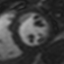
\includegraphics{src1.png}}}
\subfigure[]{\resizebox{0.15\columnwidth}{!}{\includegraphics{src1grad.png}}}
\hspace{0.15\columnwidth}
\subfigure[]{\resizebox{0.15\columnwidth}{!}{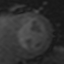
\includegraphics{src2.png}}}
\subfigure[]{\resizebox{0.15\columnwidth}{!}{\includegraphics{src2grad.png}}}


\subfigure[\hspace{1mm} \Fcs]{\resizebox{0.15\columnwidth}{!}{\includegraphics{fscalar.png}}}
\subfigure[\hspace{1mm} \Fcc]{\resizebox{0.15\columnwidth}{!}{\includegraphics{fcross.png}}}
\subfigure[\hspace{1mm} \Fcd]{\resizebox{0.15\columnwidth}{!}{\includegraphics{fscdelta.png}}}
\subfigure[\hspace{1mm} \Fcs]{\resizebox{0.15\columnwidth}{!}{\includegraphics{rscalar.png}}}
\subfigure[\hspace{1mm} \Fcc]{\resizebox{0.15\columnwidth}{!}{\includegraphics{rcross.png}}}
\subfigure[\hspace{1mm} \Fcd]{\resizebox{0.15\columnwidth}{!}{\includegraphics{rscdelta.png}}}
\itkcaption[Gradients with respect to evaluator and reference]
{The two images (a) and (c) with their respective normalized gradient fields  (b) and (d)
    are taken from a series of myocardial perfusion images where the  
    contrast changes over time due to the contrast agent passing through.
The images (e)-(g) show the gradients when image (a) is used as fixed image, and 
   the images (h)-(j) illustrate the gradient when image (c) is used as fixed image. 
The image where created with the program \code{NGFGradientMap.cpp} from the \code{Examples} directory. 
}
\label{fig:examples}
\end{figure}

In order to assess some of the properties of this metric, the two images from cardiac perfusion 
  imaging were used (Fig. \ref{fig:examples} (a), and (c)).
As can be seem from the Fig. \ref{fig:examples} (f) and (i), \Fcc (\ref{eq:cross})
  provides less gradient information.
\Fcs (\ref{eq:scalar}), and \Fcd (\ref{eq:cngf}) on the other hand provide more 
  gradient information, and they should, therefore, perform better in image registration.
Additionally, \Fcd (\ref{eq:cngf}) shows and asymmetric behavior: 
  Although Fig. \ref{fig:examples} (a) as a reference results in less gradient information then 
  using (c) (Fig. \ref{fig:examples} (g) and (j)).

However, as discussed above, \Fcs (\ref{eq:scalar})  is unstable considering gradient evaluation:
For example, when finite differences are used to evaluate the gradient $\nabla \Fcs(S,S)$ 
 (as it is implemented), the gradient that is analytically zero may evaluate to non-zero in 
  certain regions (Fig. \ref{fig:selfcost} (a)). 
\Fcc (\ref{eq:cross}), and  \Fcd (\ref{eq:cngf}), on the other hand,  are stable in that regard
  (see Fig. \ref{fig:selfcost} (b) and (c) respectively). 

\begin{figure}[h]

\center
\subfigure[\hspace{1mm} $\nabla \Fcs(S,S)$]{\resizebox{0.15\columnwidth}{!}{\includegraphics{self-scalar.png}}}
\subfigure[\hspace{1mm} $\nabla \Fcc(S,S)$]{\resizebox{0.15\columnwidth}{!}{\includegraphics{self-cross.png}}}
\subfigure[\hspace{1mm} $\nabla \Fcd(S,S)$]{\resizebox{0.15\columnwidth}{!}{\includegraphics{self-scdelta.png}}}
 
\itkcaption[Gradients of the cost function at an analytical minimum]{
  Gradients of the cost function at the analytical minimum  $R=S$ using Fig. \ref{fig:examples}(a) as image.
  Note, that the finite difference implementation of $\nabla \Fcs$ doesn't provide a zero gradient.
}
\label{fig:selfcost}
\end{figure}

\section{Testing rigid 2D registration}

In the following we present some test results of the rigid registration of a pair of images.
As Haber and Modersitzki comment in \cite{haber05}, a Gauss-Newton method would be the natural choice 
  for the optimizer, but since such optimizer is not available in the registration framework 
  of ITK, we settled for the \code{RegularStepGradientDescentOptimizer}, and 
  used \code{Rigid2DTransform} as transformation. 

The optimization parameters were set to 
\begin{itemize}
\item optimizer scales = [$\sqrt{n_x^2 + n_y^2}$, 1.0, 1.0] for an image of size $n_x \times n_y$. 
\item maximum number of iterations = 1000
\item Relaxation Factor = 0.8
\item step size $\in [\frac{1}{100}, \frac{1}{10}]$ at the lowest multiresolution level, 
  the step size boundaries will be multiplied by 2 with each change to a higher resolution, 
\end{itemize}

Note however, that the ITK implementation of the \code{RegularStepGradientDescentOptimizer}  
  is highly sensitive to a change of these parameters. 
Therefore, the results given below are by no means representative but just a proof of concept.

A 3-level multi-resolution scheme was employed, and the program to obtain the registration results 
  is implemented as \code{MultiResImageRegistration2D.cxx}
  in the \code{Examples} directory. 

\begin{table}[ph]
\center
\begin{tabular}[t]{|l|p{0.15\columnwidth}|p{0.15\columnwidth}|p{0.15\columnwidth}|p{0.15\columnwidth}|p{0.15\columnwidth}|}
\hline 
Cost & Moving & Fixed & Registered & Overlay (reg) & Overlay (unreg) \\
\hline 
\Fcd & 
\tabimage{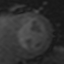
\includegraphics{src2.png}} & 
\tabimage{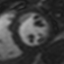
\includegraphics{src1.png}} & 
\tabimage{\includegraphics{algscdelta1-2.png}} & 
\tabimage{\includegraphics{algovscdelta1-2.png}} & 
\tabimage{\includegraphics{ovscdelta1-2.png}} \\
\hline 
\Fcs & 
\tabimage{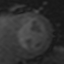
\includegraphics{src2.png}} & 
\tabimage{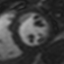
\includegraphics{src1.png}} & 
\tabimage{\includegraphics{algscalar1-2.png}} & 
\tabimage{\includegraphics{algovscalar1-2.png}} & 
\tabimage{\includegraphics{ovscalar1-2.png}} \\
\hline  
\Fcc & 
\tabimage{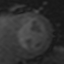
\includegraphics{src2.png}} & 
\tabimage{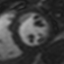
\includegraphics{src1.png}} & 
\tabimage{\includegraphics{algcross1-2.png}} & 
\tabimage{\includegraphics{algovcross1-2.png}} & 
\tabimage{\includegraphics{ovcross1-2.png}} \\
\hline 
\end{tabular}
\itkcaption[Example registrations\Fcd]{
\label{tab:highref}
  Rigid registration using different evaluation kernels and the high contrast image as reference. 
}

\vspace{12pt}

\begin{tabular}[t]{|l|p{0.15\columnwidth}|p{0.15\columnwidth}|p{0.15\columnwidth}|p{0.15\columnwidth}|p{0.15\columnwidth}|}
\hline 
Cost & Moving & Fixed & Registered & Overlay (reg) & Overlay (unreg) \\
\hline 
\Fcd & 
\tabimage{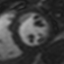
\includegraphics{src1.png}} & 
\tabimage{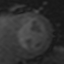
\includegraphics{src2.png}} & 
\tabimage{\includegraphics{algscdelta2-1.png}} & 
\tabimage{\includegraphics{algovscdelta2-1.png}} & 
\tabimage{\includegraphics{ovscdelta2-1.png}} \\
\hline 
\Fcs & 
\tabimage{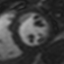
\includegraphics{src1.png}} & 
\tabimage{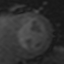
\includegraphics{src2.png}} & 
\tabimage{\includegraphics{algscalar2-1.png}} & 
\tabimage{\includegraphics{algovscalar2-1.png}} & 
\tabimage{\includegraphics{ovscalar2-1.png}} \\
\hline  
\Fcc & 
\tabimage{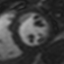
\includegraphics{src1.png}} & 
\tabimage{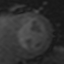
\includegraphics{src2.png}} & 
\tabimage{\includegraphics{algcross2-1.png}} & 
\tabimage{\includegraphics{algovcross2-1.png}} & 
\tabimage{\includegraphics{ovcross2-1.png}} \\
\hline 
\end{tabular}
\itkcaption[Example registrations\Fcd]{
\label{tab:lowref}
  Rigid registration using different evaluation kernels and the low contrast image as reference. 
}
\end{table}

In the first case (Table \ref{tab:highref}), we selected image Fig. \ref{fig:examples} (a) 
  as reference and the  Fig. \ref{fig:examples} (b) as moving image. 
As the colored overlay of the registered moving and the fixed image show, 
  all three cost functions perform equally well in this setting and with the given optimization parameters.

However, using Fig. \ref{fig:examples} (b) image as fixed and the high contrast image as moving image 
  results in a different picture: 
Applying \Fcd as registration criterion performs well, but using  
  \Fcc or \Fcs as evaluators kernels doesn't result in proper registration (Table \ref{tab:lowref}). 

\section{Software}

\subsection{Requirements}
To only use the cost function and run the registration examples the following software is required:
\begin{itemize}
  \item  Insight Toolkit $\ge$ 3.10, 
  \item  CMake $\ge$ 2.6, 
  \item  A C++ compiler. It is highly recommended to use a compiler that supports partial 
    template specialization.
\end{itemize}

For running the tests, one will also need 
\begin{itemize}
\item  BOOST $\ge$ 1.34.1
\end{itemize}
for its testing framework. 

Further software is required to create this document:
\begin{itemize}
\item LaTeX 
\item GNU Make 
\end{itemize}

\section{Closing notes}

Currently, the image metric does not support masks. 
In addition, some of the code needs to be reworked to use facilities provided by ITK to support 
  multi-threading of the metric evaluation and properly triggering the \code{Update} function.
Finally, with the current generic implementation using a B-Spline based transformation 
  model results in very long run-times.

\section*{Acknowledgment}

This study was partially supported by research projects  TIN2007-68048-C02-01, 
  CDTI-CDTEAM and SINBAD (PS-010000-2008-1) from Spain's Ministry of Science and Innovation.
Image data was provided with the support of the Intramural Research Program of the 
  NIH, National Heart, Lung and Blood Institute.

\bibliographystyle{plain}
\bibliography{InsightJournal}

\end{document}

